% VerdeAI ISO clause data structure — legacy free-text requirements vs. slot schema.
% Standalone: compiles alone to one cropped page.
\documentclass[tikz, border=6mm]{standalone}
\usetikzlibrary{shapes.geometric, arrows.meta, positioning, calc}

\definecolor{inkcolor}{HTML}{17241B}
\definecolor{mutedtext}{HTML}{4D5D4F}
\definecolor{decisionfill}{HTML}{E6D3A3}
\definecolor{processfill}{HTML}{BFD3BC}
\definecolor{oldfill}{HTML}{E3B7B0}
\definecolor{newfill}{HTML}{9FC2B2}
\definecolor{fieldfill}{HTML}{EDEFEA}

\begin{document}
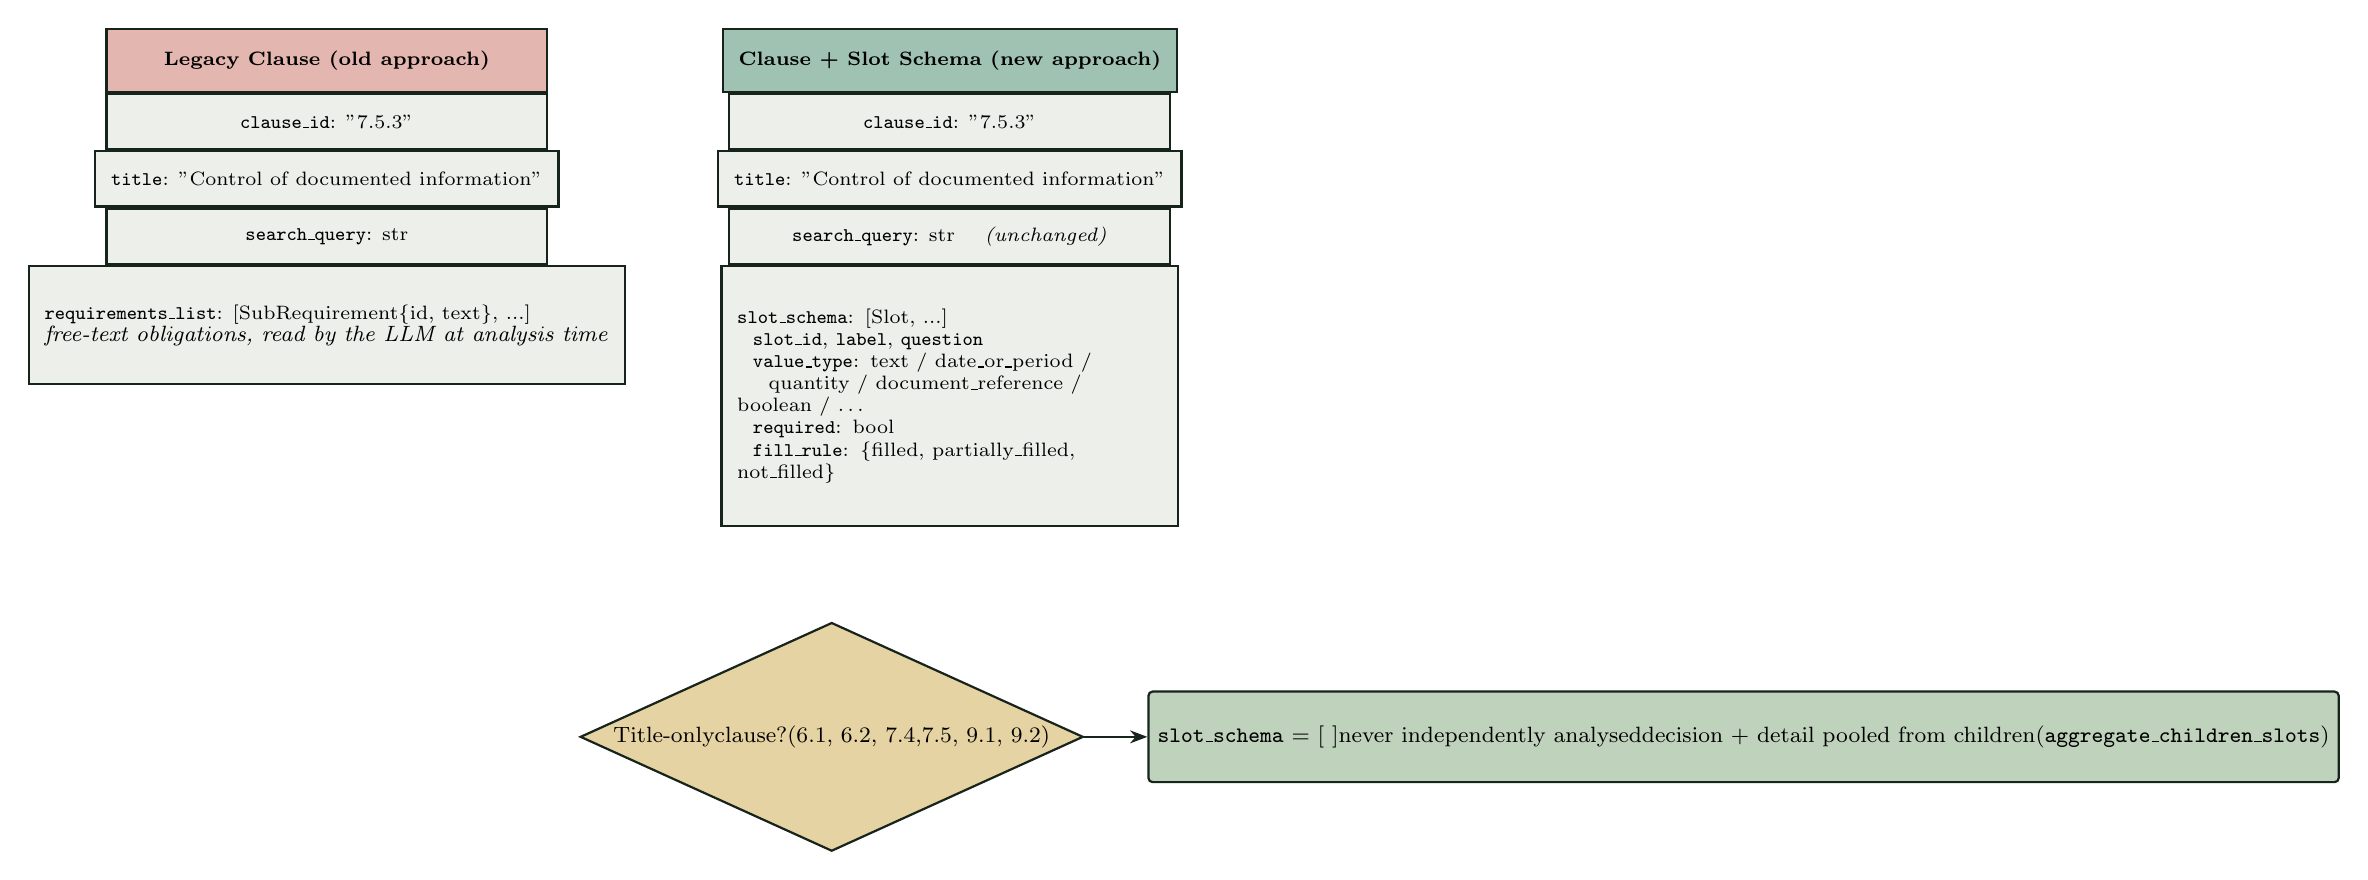
\begin{tikzpicture}[every node/.style={font=\footnotesize}, thick]

\tikzset{
  flowline/.style={-{Stealth[length=2.2mm]}, inkcolor},
  decision/.style={diamond, draw=inkcolor, fill=decisionfill, aspect=2.4,
    inner sep=1pt, minimum width=2.5cm, minimum height=1.35cm},
  process/.style={rectangle, rounded corners=1.5pt, draw=inkcolor, fill=processfill,
    minimum width=2.6cm, minimum height=1.15cm},
  annotation/.style={rectangle, rounded corners=2pt, draw=mutedtext, dashed, fill=white,
    text width=4.4cm, font=\tiny, align=left, inner sep=2mm},
  recordbox/.style={rectangle, draw=inkcolor, fill=fieldfill,
    minimum width=5.6cm, minimum height=0.7cm, font=\scriptsize, align=left,
    inner sep=2mm, anchor=north west},
  rechead/.style={rectangle, draw=inkcolor,
    minimum width=5.6cm, minimum height=0.8cm, font=\bfseries\scriptsize,
    align=center, inner sep=2mm, anchor=north west},
}

% ---- left: legacy clause record ----
\node[rechead, fill=oldfill] (oldhead) at (0,0) {Legacy Clause (old approach)};
\node[recordbox, below=0mm of oldhead]      (o1) {\texttt{clause\_id}: "7.5.3"};
\node[recordbox, below=0mm of o1]           (o2) {\texttt{title}: "Control of documented information"};
\node[recordbox, below=0mm of o2]           (o3) {\texttt{search\_query}: str};
\node[recordbox, below=0mm of o3, minimum height=1.5cm]
  (o4) {\texttt{requirements\_list}: [SubRequirement\{id, text\}, ...]\\
         \footnotesize\textit{free-text obligations, read by the LLM at analysis time}};
% ---- right: new slot-schema clause record ----
\node[rechead, fill=newfill, right=2.2cm of oldhead] (newhead) {Clause + Slot Schema (new approach)};
\node[recordbox, below=0mm of newhead]      (n1) {\texttt{clause\_id}: "7.5.3"};
\node[recordbox, below=0mm of n1]           (n2) {\texttt{title}: "Control of documented information"};
\node[recordbox, below=0mm of n2]           (n3) {\texttt{search\_query}: str \quad\textit{(unchanged)}};
\node[recordbox, below=0mm of n3, minimum height=3.3cm, text width=5.4cm]
  (n4) {\texttt{slot\_schema}: [Slot, ...] \newline
  \hspace*{2mm}\texttt{slot\_id}, \texttt{label}, \texttt{question} \newline
  \hspace*{2mm}\texttt{value\_type}: text / date\_or\_period / \newline
  \hspace*{4mm}quantity / document\_reference / boolean / \dots \newline
  \hspace*{2mm}\texttt{required}: bool \newline
  \hspace*{2mm}\texttt{fill\_rule}: \{filled, partially\_filled, not\_filled\}};

\node[decision, fill=decisionfill, below=12mm of n4, xshift=-1.5cm,
      minimum width=2.6cm, minimum height=1.2cm, aspect=2.2] (titleonly)
  {Title-only\\clause?\\\footnotesize(6.1, 6.2, 7.4,\\7.5, 9.1, 9.2)};
\node[process, right=8mm of titleonly, minimum width=4.6cm]
  (noschema) {\texttt{slot\_schema} = [ ] \\ never independently analysed \\
  decision + detail pooled from children \\ (\texttt{aggregate\_children\_slots})};
\draw[flowline] (titleonly) -- (noschema);

\end{tikzpicture}
\end{document}
